% !LW recipe = pdflatex (quick build)
\documentclass[tikz,border=3pt]{standalone}
\usepackage{tikz}
\usetikzlibrary{calc}

\definecolor{inboundfill}{RGB}{216,235,211}
\definecolor{outboundfill}{RGB}{247,218,205}
\definecolor{storagefilltwo}{RGB}{207,230,249}
\definecolor{storagefillthree}{RGB}{221,239,252}
\definecolor{storagefillfive}{RGB}{198,224,247}
\definecolor{storagefillsix}{RGB}{214,234,251}
\definecolor{storagefillseven}{RGB}{187,218,244}
\definecolor{storagefilleight}{RGB}{229,244,254}

\begin{document}

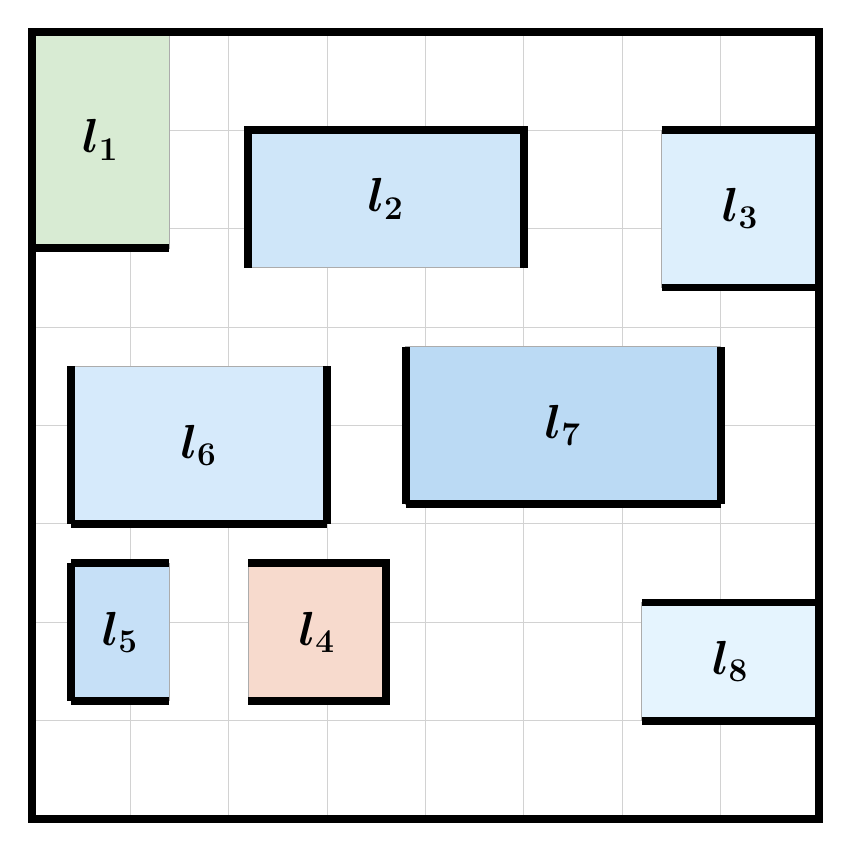
\begin{tikzpicture}[x=0.25cm,y=0.25cm]

% Each region is specified as:
% \region{label}{x}{y}{width}{height}{fill}
\newcommand{\region}[6]{%
  \filldraw[fill=#6, draw=gray!65, line width=0.35pt]
    (#2,#3) rectangle ++(#4,#5);
  \node[font=\fontfamily{ptm}\fontsize{17}{19}\selectfont\bfseries\boldmath]
    at ($(#2,#3)+(#4/2,#5/2)$) {$l_{#1}$};
}

\tikzset{
  region wall/.style={
    draw=black,
    line width=0.10cm,
    line cap=butt,
    line join=miter
  }
}

% Major grid lines every 5 units.
\foreach \v in {0,5,...,40}{
  \draw[gray!35, line width=0.25pt] (\v,0) -- (\v,40);
  \draw[gray!35, line width=0.25pt] (0,\v) -- (40,\v);
}

% Regions.
\region{1}{0}{29}{7}{11}{inboundfill}
\region{2}{11}{28}{14}{7}{storagefilltwo}
\region{3}{32}{27}{8}{8}{storagefillthree}
\region{4}{11}{6}{7}{7}{outboundfill}
\region{5}{2}{6}{5}{7}{storagefillfive}
\region{6}{2}{15}{13}{8}{storagefillsix}
\region{7}{19}{16}{16}{8}{storagefillseven}
\region{8}{31}{5}{9}{6}{storagefilleight}

% Region l_1: only the bottom wall is retained.
\draw[region wall] (0,29) -- (7,29);

% Region l_2: doorway on the bottom.
\draw[region wall] (11,28) -- (11,35) -- (25,35) -- (25,28);

% Region l_3: doorway on the left; the right side uses the outer frame.
\draw[region wall] (32,27) -- (40,27);
\draw[region wall] (32,35) -- (40,35);

% Region l_4: doorway on the left.
\draw[region wall] (11,13) -- (18,13) -- (18,6) -- (11,6);

% Region l_5: doorway on the right.
\draw[region wall] (2,6) -- (7,6);
\draw[region wall] (2,13) -- (7,13);
\draw[region wall] (2,6) -- (2,13);

% Region l_6: doorway on the top.
\draw[region wall] (2,15) -- (15,15);
\draw[region wall] (2,15) -- (2,23);
\draw[region wall] (15,15) -- (15,23);

% Region l_7: doorway on the top.
\draw[region wall] (19,16) -- (35,16);
\draw[region wall] (19,16) -- (19,24);
\draw[region wall] (35,16) -- (35,24);

% Region l_8: doorway on the left; the right side uses the outer frame.
\draw[region wall] (31,5) -- (40,5);
\draw[region wall] (31,11) -- (40,11);

% Complete black outer frame.
\draw[black, line width=0.10cm] (0,0) rectangle (40,40);

\end{tikzpicture}

\end{document}
